\documentclass[t, screen, aspectratio=43]{beamer}
\usepackage[T1]{fontenc}
\usepackage[utf8]{inputenc}
\usepackage{epsf}
\usepackage{graphicx}
\usepackage{geometry}
\usepackage{tabularx}
\usepackage[table]{colortbl}
\usepackage{xcolor}
\usepackage{soul}
\usepackage[normalem]{ulem}
\usepackage{tikz}
\usepackage{subcaption}
\usepackage{hyperref}
% Use the NTNU-temaet for beamer 
% \usetheme[style=ntnu|simple|vertical|horizontal, 
%     language=bm|nn|en, 
%     smalltitle, 
%     city=all|trondheim|alesund|gjovik]{ntnu2017}
\usetheme[style=helvet,language=en]{ntnu2017}

\usepackage[english]{babel}
\usepackage[style=numeric,backend=biber,natbib=false,sorting=none]{biblatex}

\title[Short title]{Ultra low power integer-N ADPLL}
\subtitle{Master's thesis project - meeting 5}
\author[C Nielsen]{Cole Nielsen}
\institute[NTNU]{Department of Electronic Systems, NTNU}
\date{14 February 2020 $\heartsuit$ (calendar week 7)}
%\date{} % To have an empty date

\addbibresource{example.bib} % Add bibliography database

% Set the reference style to numeric.
% See here: http://tex.stackexchange.com/questions/68080/beamer-bibliography-icon
\setbeamertemplate{bibliography item}[text] 

% Set bibliography fonts to a small size.
\renewcommand*{\bibfont}{\footnotesize}

\usepackage{tikz}
\usepackage{enumitem}
\newcommand*\mycirc[1]{%
\begin{tikzpicture}[baseline=(C.base)]
	\node[draw,circle,inner sep=1pt,minimum size=3ex](C){#1};
\end{tikzpicture}}


\begin{document}

\begin{frame}
	\titlepage%
\end{frame}

% Alternatively, special title page command to get a different background
% \ntnutitlepage

% #############################################################################
% This week
% #############################################################################

\begin{frame}
	\frametitle{Overview}
	\begin{block}{For this week...}
		\begin{enumerate}[itemsep=4pt,label=\protect\mycirc{\arabic*}]
			\scriptsize
			\item Some more with synchronous counter.
			\item Bang bang phase detector.
			\item New {\color{blue}\href{https://github.com/nielscol/thesis_presentations}{\underline{Github repo}}} for presentations.
		\end{enumerate} 
	\end{block}	
\end{frame}


% #############################################################################
% This week
% #############################################################################


% #############################################################################
% Physical limits
% #############################################################################

\begin{frame}
	\frametitle{DFF Architectures}
	\begin{block}{True single phase clock.}
	\tiny
	\begin{itemize}[itemsep=4pt,label=\protect---]
		\item True single phase clock (TSPC) advantageous for low power.
		\item If TSPC is too slow, enhanced TSPC (e-TSPC) is essentially the fastest possible DFF architecture in CMOS. However, power consumption is horrendous as it results in direct conduction paths from rail to rail on the order of 25\% of the time if used as BB-PD.

	\end{itemize}
	% \vspace{-3em}
	\begin{figure}[htb!]
	    \centering
	    \begin{subfigure}{0.5\textwidth}
	        \centering
	        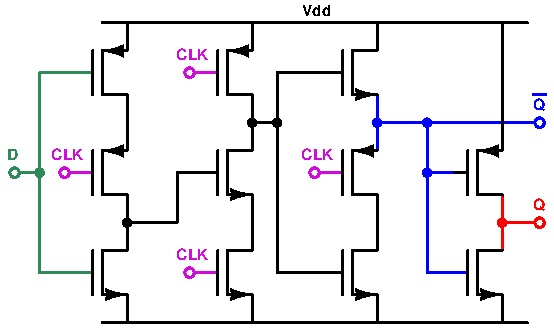
\includegraphics[width=0.8\textwidth, angle=0]{tspc_dff.pdf}
	        \caption{TSPC DFF}
	    \end{subfigure}%
	    \begin{subfigure}{0.5\textwidth}
	        \centering
	        \center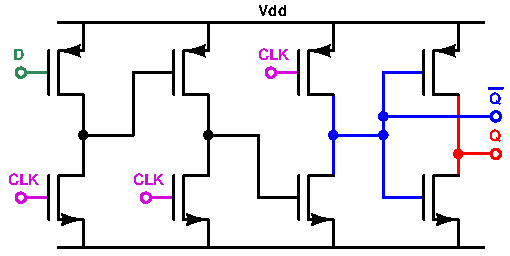
\includegraphics[width=0.8\textwidth, angle=0]{etspc_dff.pdf}
	        \caption{e-TSPC DFF}
	    \end{subfigure}
	    % \caption{Approximate model for ring oscillator inverter delay cell.}
	\end{figure}

	\end{block}	
\end{frame}

\begin{frame}
	\frametitle{Synchronous counter architecture}
	\begin{block}{For real this time.}
	\tiny
	\begin{itemize}[itemsep=4pt,label=\protect---]
		\item Only tested ripple (asynchronous) counter last time. 
		\item Implement T flip-flop with XOR gate, AND carry logic. Logic implemented as NAND2 only, with all FETS 200nm/20nm. 
		\item Necessary to ensure that incorrect value isn't sampled, which is possible with asynchronous during ripple period. Penalty: 50 NAND2 gates, all FF's must be clocked every input cycle, i.e. more power than async.
	\end{itemize}
	% \vspace{-3em}
	\begin{figure}[htb!]
	        \centering
	        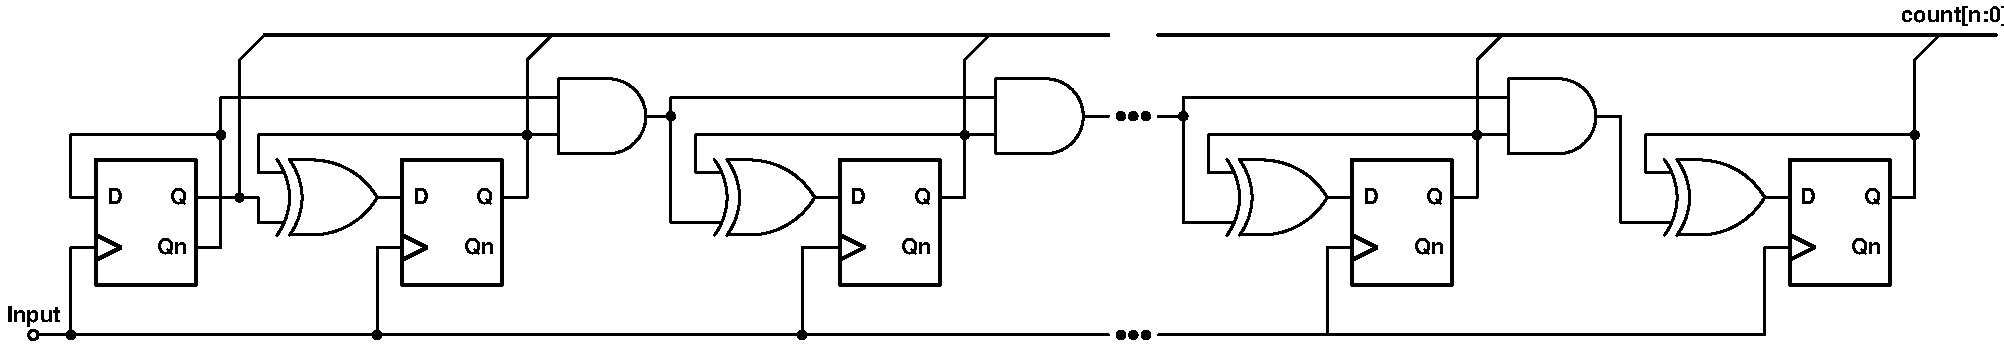
\includegraphics[width=1\textwidth, angle=0]{sync_counter.pdf}
	    % \caption{Approximate model for ring oscillator inverter delay cell.}
	\end{figure}

	\end{block}	
\end{frame}

\begin{frame}
	\frametitle{8 bit ripple async. counter power}
	\begin{block}{Power consumption under swept conditions.}
	\tiny
	\begin{itemize}[itemsep=4pt,label=\protect---]
		\item Chain of 8 DFFs whose output clocks the next respective FF in the chain.
		\item Tested (W/L) = \{100n/20, 200n/20\}, $C_{min}$ = \{10, 100\} aF, V$_{dd} \in [0.3, 0.8]$ V. 
		\item TSPC has favorable power consumption. e-TSPC is terrible on the other hand, but is less sensitive to loading.

	\end{itemize}
	% \vspace{-3em}
	\begin{figure}[htb!]
	    \centering
	    \begin{subfigure}{0.5\textwidth}
	        \centering
	        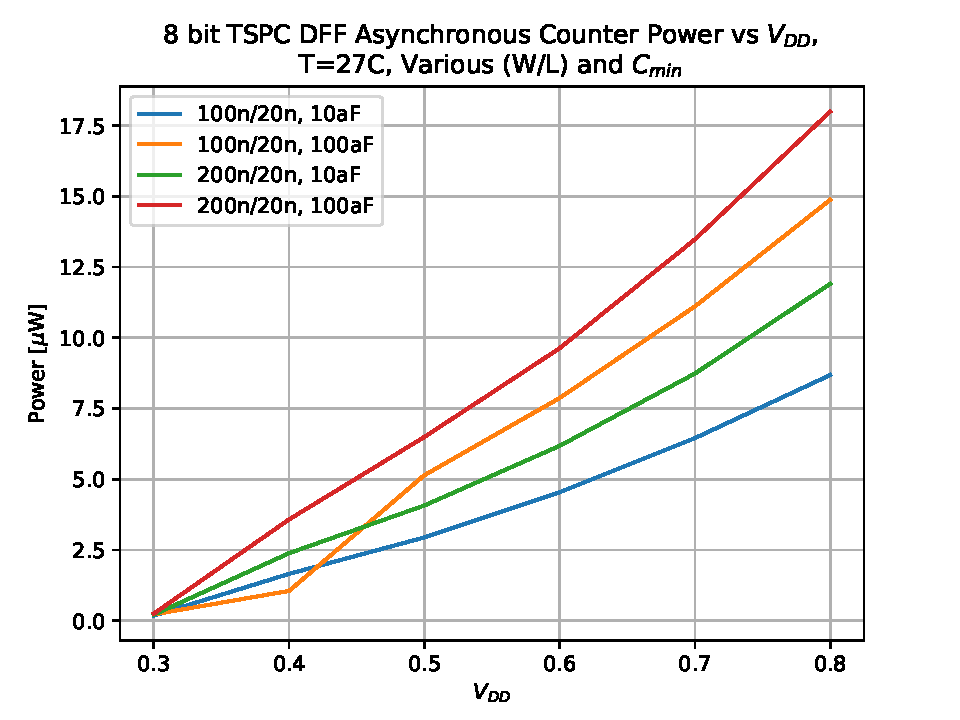
\includegraphics[width=1\textwidth, angle=0]{tspc_counter_power.pdf}
	    \end{subfigure}%
	    \begin{subfigure}{0.5\textwidth}
	        \centering
	        \center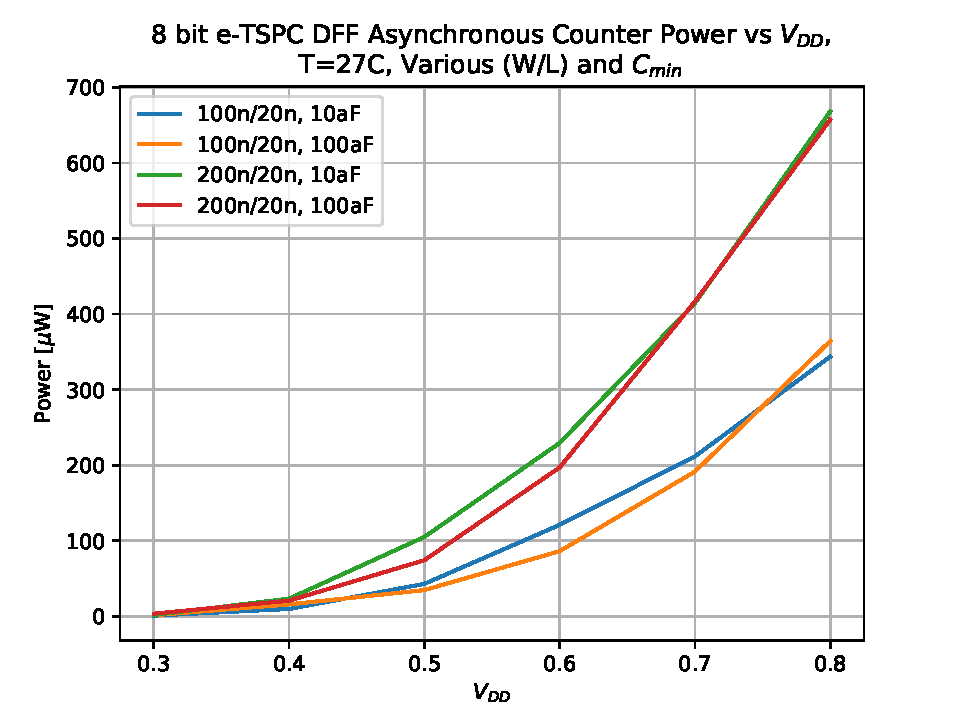
\includegraphics[width=1.0\textwidth, angle=0]{etspc_counter_power.pdf}
	    \end{subfigure}
	    % \caption{Approximate model for ring oscillator inverter delay cell.}
	\end{figure}

	\end{block}	
\end{frame}

\begin{frame}
	\frametitle{8 bit synchronous counter power}
	\begin{block}{Power consumption under swept conditions.}
	\tiny
	\begin{itemize}[itemsep=4pt,label=\protect---]
		\item Tested (W/L) = \{100n/20, 200n/20\}, $C_{min}$ = \{10, 100\} aF, V$_{dd} \in [0.3, 0.8]$ V. 
		\item Minimizing capacitance is most favorable for power. However, it is expected that 50 $\mu$W of counter power will only increase average power by $<< 1 \mu$W. So all circumstance tested here appear acceptable.
	\end{itemize}
	% \vspace{-3em}
	\begin{figure}[htb!]
	        \centering
	        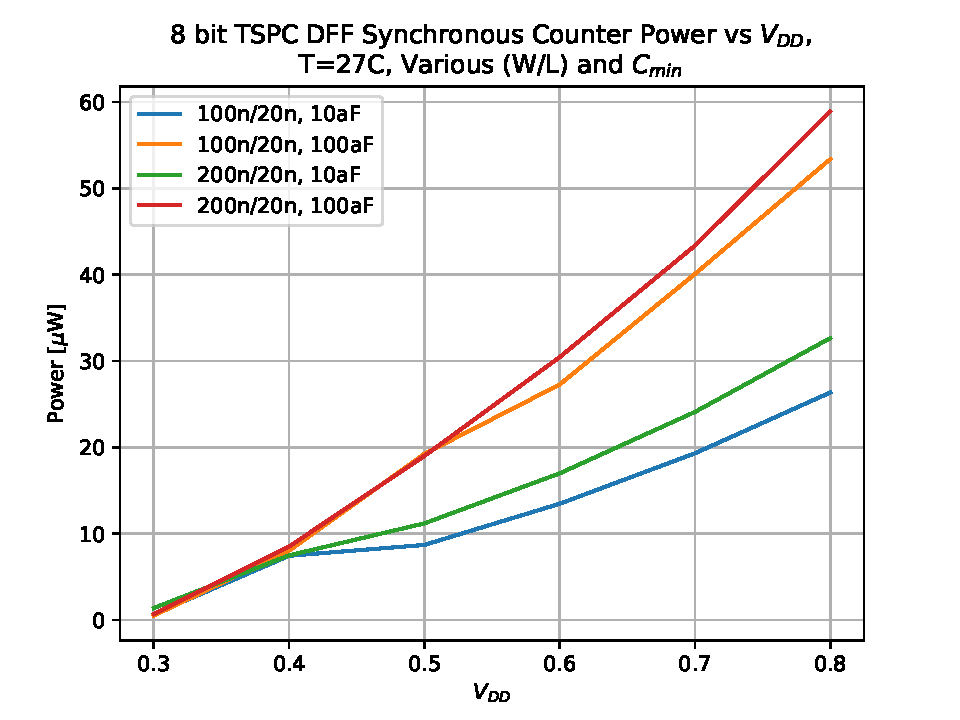
\includegraphics[width=0.5\textwidth, angle=0]{tspc_sync_counter_power.pdf}
	    % \caption{Approximate model for ring oscillator inverter delay cell.}
	\end{figure}

	\end{block}	
\end{frame}



\begin{frame}
	\frametitle{Synchronous counter output}
	\begin{block}{800 mV Vdd}
	\tiny
	All edges occur within a time interval of 80ps. 54 $\mu$W power with 100 aF $C_{min}$
	\begin{figure}[htb!]

	        \center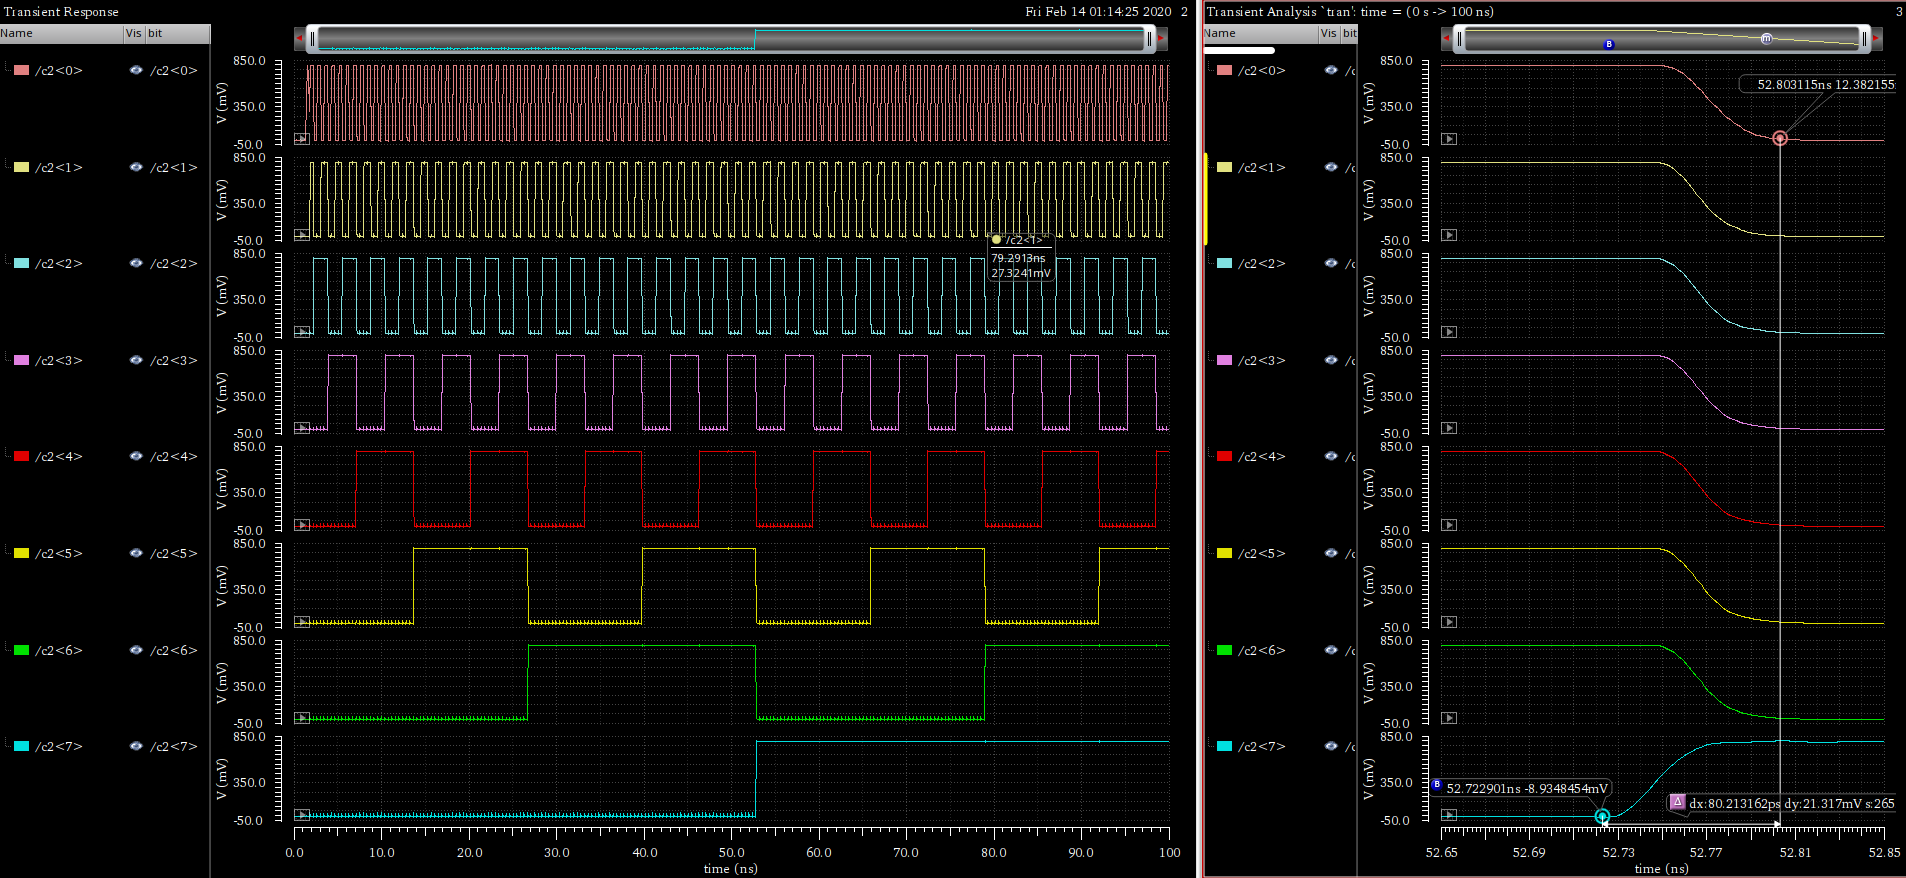
\includegraphics[width=0.9\textwidth, angle=0]{sync_counter_timing.png}
	\end{figure}
	\end{block}	
\end{frame}

\begin{frame}
	\frametitle{Noisy BB-PD Model.}
	\begin{block}{Introduction of timing jitter to model.}
	\tiny
	\begin{itemize}[itemsep=4pt,label=\protect---]
		\item Uncorrelated / stochastic processes in a BB-PD result in the $\mathbb{E}[Z]$ with respect to input timing difference $\Delta t_{xy}$ to deviate from an ideal step response.
		\item $d\mathbb{E}[Z]/d\Delta t_{xy}$ results in a timing jitter probability distribution P(T=$\Delta t_{xy}$). The variance of this distribution on random jitter variable T, $\mathrm{Var}[T] = \sigma_{t,j}^2$, is the jitter power.
	\end{itemize}

	\begin{figure}[htb!]
	    \centering
		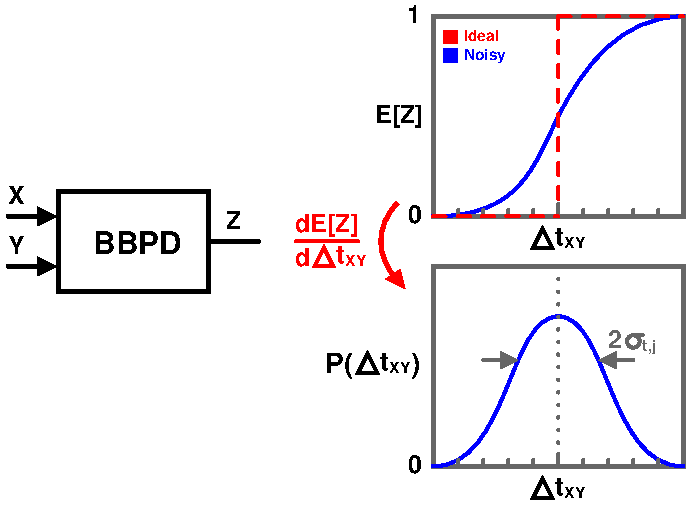
\includegraphics[width=0.45\textwidth, angle=0]{bbpd_jitter.pdf}
	\end{figure}
	\end{block}	
\end{frame}

\begin{frame}
	\frametitle{Simulation of BB-PD.}
	\begin{block}{Simulation with TSPC DFF - Output expectation vs input delta.}
	\tiny
	\begin{itemize}[itemsep=4pt,label=\protect---]
		\item Utilized TSPC DFF, with inverter buffers (FETs sized 200n/20n) for clock and data buffers.
		\item Sweep delay between inputs, calculating the expect value of the output for 100 bits. Transient noise simulated (up to 100 GHz), and the inital state of the FF is set to be high 50x and low 50x to include hysteresis effects. 
		\item V$_{DD} \in$ \{0.5, 0.8\} V and (W/L) $\in$ \{100n/20n, 200n/20n\} tested. 100 aF added to every node.
		\item \textbf{Resulting CDFs of the input time delta versus output expectation are below.}
	\end{itemize}
	\vspace{-2em}
	\begin{figure}[htb!]
	    \centering
		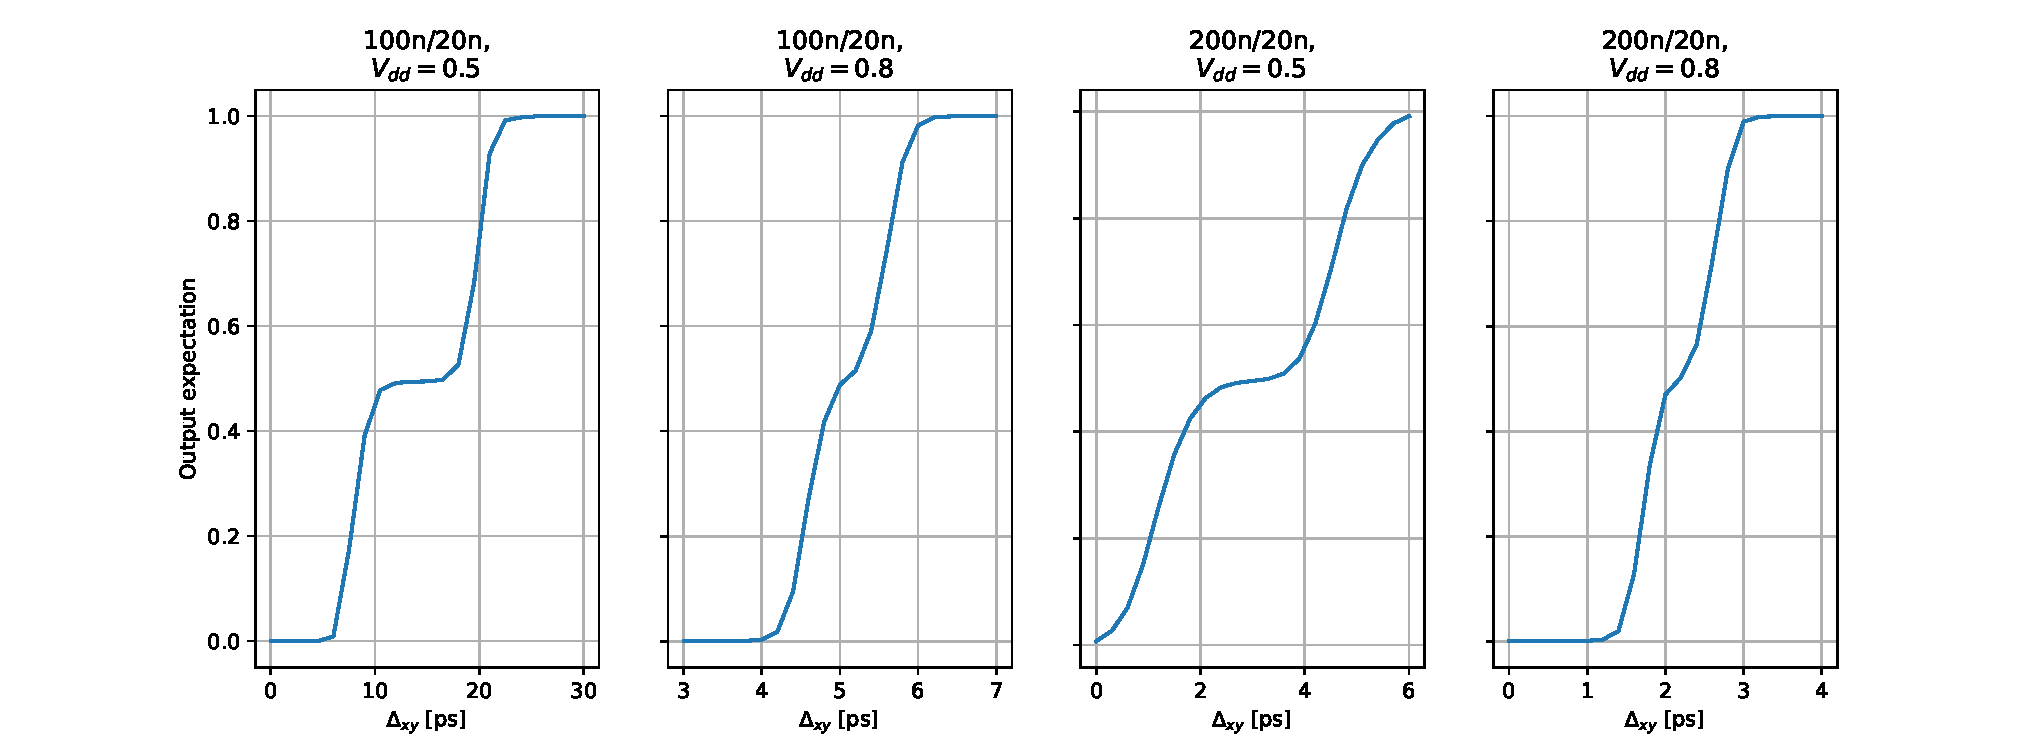
\includegraphics[width=1\textwidth, angle=0]{cdfs.pdf}
	\end{figure}
	\end{block}	
\end{frame}

\begin{frame}
	\frametitle{Simulation of BB-PD.}
	\begin{block}{Simulation with TSPC DFF - Jitter distributions.}
	\tiny
	\begin{itemize}[itemsep=4pt,label=\protect---]
		\item Jitter PDFs are bimodal from hysteresis of DFF. 
		\item Increasing (W/L) or $V_{DD}$ both impact jitter favorably.
		\item \textbf{The jitter PDF (computed from the CDFs) of the input time delta versus output expectation are below. (Delays are removed)}
	\end{itemize}
	\vspace{-2em}
	\begin{figure}[htb!]
	    \centering
		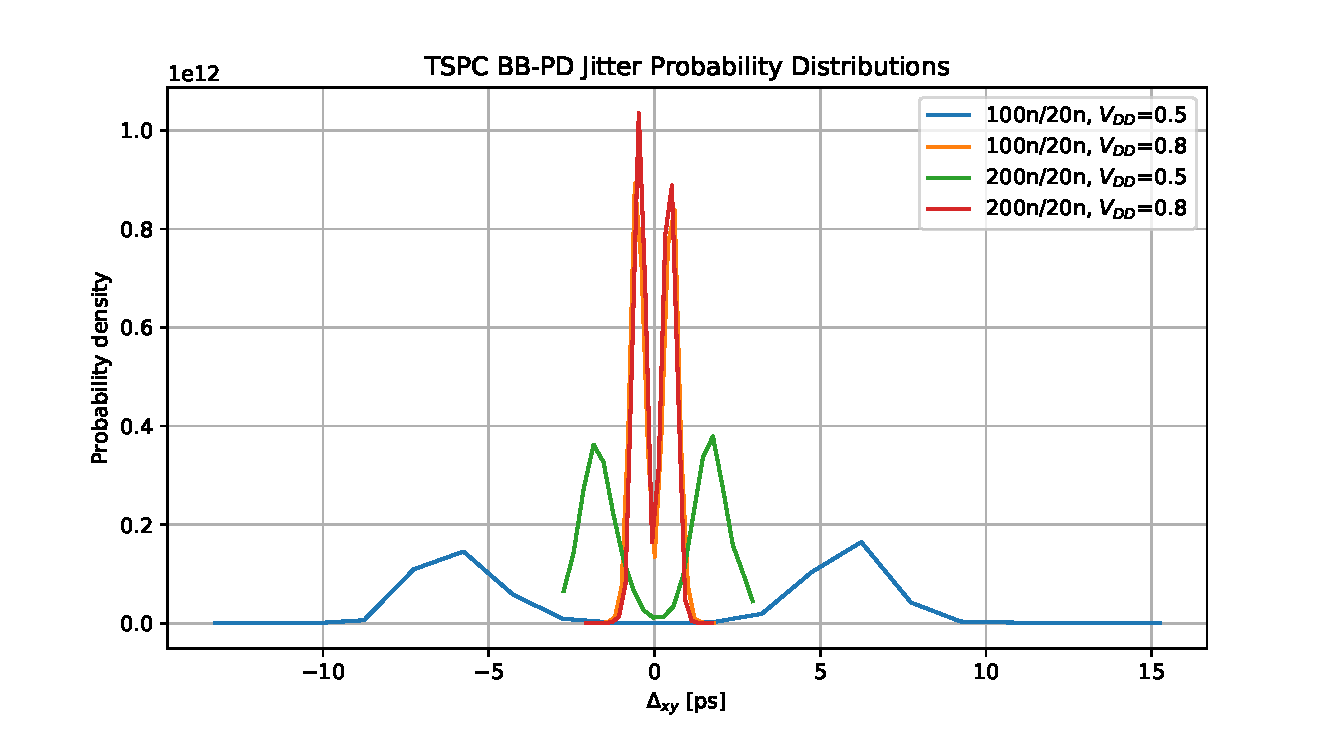
\includegraphics[width=0.7\textwidth, angle=0]{jitter_pdfs.pdf}
	\end{figure}
	\end{block}	
\end{frame}

\begin{frame}
	\frametitle{Simulation of BB-PD.}
	\begin{block}{Tabularized results.}
		\tiny
		Requirements were $<$ 10 $\mu$W for the BB-PD, and its RMS jitter to be <12 ps for 17 dB CNR or < 8 ps for 20 dB CNR.
		\begin{table}[h!]
			\centering
			\def\arraystretch{1.5}		
			\setlength\arrayrulewidth{0.75pt}
			\setlength{\tabcolsep}{1em} % for the horizontal padding
			\begin{tabular}{|c|c|c|c|c|c|c|}
				\hline 
				\rule[-1ex]{0pt}{2.5ex} \cellcolor{gray!40}\textbf{(W/L)} & \cellcolor{gray!40}\textbf{Supply [V]} & \cellcolor{gray!40}\textbf{RMS jitter [ps]}& \cellcolor{gray!40}\textbf{Delay [ps]} & \cellcolor{gray!40}\textbf{DFF [$\mu$W]} & \cellcolor{gray!40}\textbf{Buffer [$\mu$W]} & \cellcolor{gray!40}\textbf{Total Power [$\mu$W]}\\ 
				\hline 
				\rule[-1ex]{0pt}{2.5ex} 100n/20n  & 0.5 & 6.01 & 13.3 & 1.64 & 1.595 & 3.236 \\ 
				\hline 
				\rule[-1ex]{0pt}{2.5ex} 100n/20n  & 0.8 & 0.832 & 4.99 & 3.942 & 4.195 & 8.136 \\ 
				\hline 
				\rule[-1ex]{0pt}{2.5ex} 200n/20n  & 0.5 & 1.776 & 2.73 & 2.215 & 1.81 & 4.025 \\ 
				\hline 
				\rule[-1ex]{0pt}{2.5ex} 200n/20n  & 0.8 & 0.496 & 2.072 & 4.591 & 4.518 & 9.109 \\ 
				\hline 
			\end{tabular} 
			% \caption{Assigned specifications for branch line hybrid design.}
			% \label{asgn_specs}
		\end{table}   
		{\color{red}\textbf{All four scenarios tested here pass the requirements.}} This will have to be re-evaluated post layout and with supply noise, however.
	\end{block}    
\end{frame}

\begin{frame}
	\frametitle{Noisy BB-PD Model. \color{red}RECAP}
	\begin{block}{Linearized noisy BB-PD model.}
	\tiny
	\begin{figure}[htb!]
	    \centering
		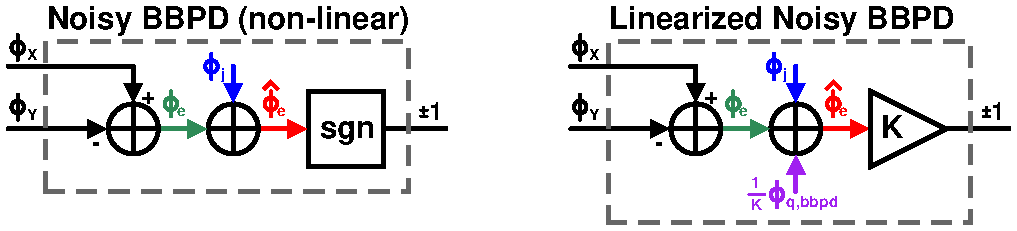
\includegraphics[width=0.55\textwidth, angle=0]{bbpd_noise_linearized.pdf}
	\end{figure}
	\begin{itemize}[itemsep=4pt,label=\protect---]
		\item BB-PD is non-linear, however with a stationary input $\phi_e$ with power  $\sigma^2_{\phi_e}$, its gain can be linearized [1] as:
		\tiny
		\begin{equation}
			K = \sqrt{\frac{2}{\pi}}\cdot\frac{1}{\sigma_{\phi_e}}
		\end{equation}
		\item The output has power $\sigma^2_{\phi_Z}$ = 1 = $K^2\sigma^2_{\phi_e}$ + $\sigma^2_{\phi_{q,bbpd}}$
		\item $\phi_{q,bbpd}$ is a error noise power inherent to the BB-PD. 
		\begin{equation}
			\sigma^2_{\phi_{q,bbpd}} = 1 - \frac{2}{\pi}
		\end{equation}
	\end{itemize}

	\end{block}	
\end{frame}

\begin{frame}
	\frametitle{Noisy BB-PD Model. \color{red}RECAP}
	\begin{block}{Linearized noisy BB-PD model (continued).}
	\tiny
	\begin{figure}[htb!]
	    \centering
		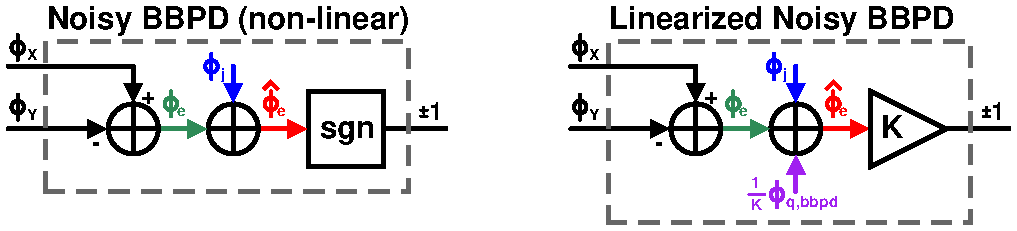
\includegraphics[width=0.55\textwidth, angle=0]{bbpd_noise_linearized.pdf}
	\end{figure}
	\begin{itemize}[itemsep=4pt,label=\protect---]
		\item Referring $\phi_{q,bbpd}$ to be before gain K, results in a total phase noise power for the BB-PD (assuming all noise sources uncorrelated):
		\tiny
		\begin{equation}
			\sigma^2_{\phi_{n,BBPD}} =   \left(\frac{\pi}{2}-1\right)\sigma^2_{\phi_e} + \frac{\pi}{2}\sigma^2_{\phi_j}
		\end{equation}
		\item If the BB-PD is connected directly to oscillator output, $\sigma^2_{\phi_e}$ = $\sigma^2_{\phi_n}$, i.e. the PLL output phase noise. The spectral density of the BB-PD phase noise is then:
		\begin{equation}
			S_{\phi_{n,BBPD}} = \frac{\sigma^2_{\phi_{n,BBPD}}}{f_{ref}} =  \frac{\left(\frac{\pi}{2}-1\right)\sigma^2_{\phi_n} + \frac{\pi}{2}\sigma^2_{\phi_j}}{f_{ref}}
		\end{equation}
	\end{itemize}

	\end{block}	
\end{frame}

\begin{frame}
	\frametitle{BB-PD PLL Optimization. \color{red}RECAP}
	\begin{block}{Approximate model for phase noise and optimal bandwidth.}
	\tiny
	\begin{itemize}[itemsep=4pt,label=\protect---]
		\item It is observed that PLL phase noise spectrum is approximately Lorentzian (except for peaking and flicker noise components). Given BB-PD noise PSD of $S_{\phi_{n,BBPD}}$, and an oscillator with noise PSD $S_{\phi_{n,osc}}(\Delta f)$, the optimal bandwidth for minimum noise power is:
		\tiny
		\begin{equation}
			BW_{opt} =  \sqrt{\frac{S_{\phi_{n,osc}}(\Delta f)}{S_{\phi_{n,BBPD}}}}\Delta f
		\end{equation}
		\item The total PLL output phase noise with optimal bandwidth is then:
		\tiny
		\begin{equation}
			\sigma^2_{\phi_{n,opt}} =   \pi\sqrt{\phi_{n,osc}(\Delta f)S_{\phi_{n,BBPD}}}\Delta f
		\end{equation}
	\end{itemize}
	\vspace{-3em}
	\begin{figure}[htb!]
	    \centering
	    \begin{subfigure}{0.33\textwidth}
	        \centering
	        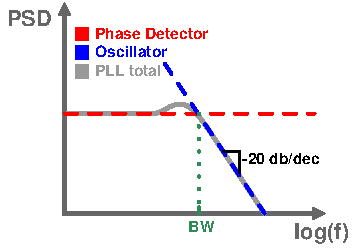
\includegraphics[width=1\textwidth, angle=0]{pll_spectrum_lorentzian.pdf}
	    \end{subfigure}%
	    \begin{subfigure}{0.33\textwidth}
	        \centering
	        \center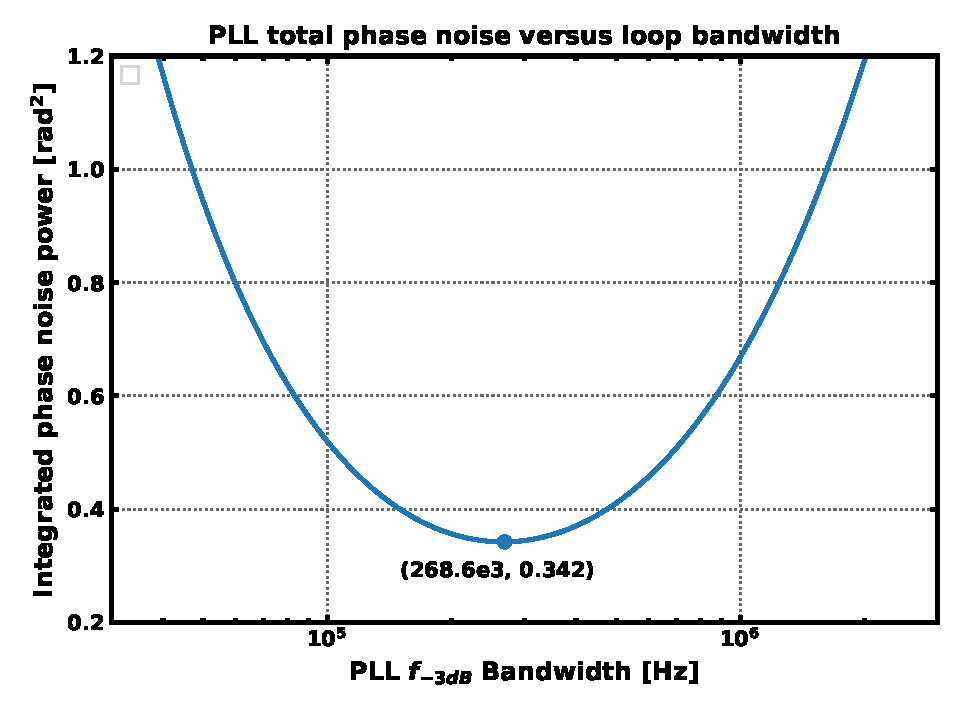
\includegraphics[width=1.0\textwidth, angle=0]{bandwidth_vs_pn.pdf}
	    \end{subfigure}
	    % \caption{Approximate model for ring oscillator inverter delay cell.}
	\end{figure}

	\end{block}	
\end{frame}

\begin{frame}
	\frametitle{BB-PD PLL Optimization. \color{red}RECAP}
	\begin{block}{BB-PD Jitter constraint with fixed BW and f$_{ref}$ relationship.}
	\tiny
	\begin{itemize}[itemsep=4pt,label=\protect---]
		\item Using the findings for BB-PD noise PSD, assumption of Lorentzian spectrum, and constraint that BW = $\alpha f_{ref}$ (recommended $\alpha$$<$0.1 [2], rule of thumb since ancient PLL days). Given oscillator center frequency $f_c$, BB-PD jitter is constrained:
		\tiny
		\begin{equation}
			\sigma_{t_j} \leq \frac{\sigma_{\Phi_n}}{2\pi f_c}\sqrt{\frac{2}{\pi}\left(\frac{1}{\pi\alpha} - \frac{\pi}{2} + 1\right)} = \frac{\sigma_{\Phi_n}}{2\pi f_c}\beta(\alpha)
		\end{equation}
		\item $\beta(\alpha=0.1)$ = 1.28, $\beta(\alpha=0.05)$ = 1.92.
		\item Using my PLL specifications ($f_c$ = 2.448 GHz, CNR = -$\sigma_{\Phi_n}$ = 17 dB, $\alpha=0.1$), {\color{red}\textbf{$\sigma_{t,j}\leq 11.8 $ ps}}
	\end{itemize}


	\end{block}	
	\begin{block}{BB-PD optimal Jitter.}
	\tiny
	\begin{itemize}[itemsep=4pt,label=\protect---]
		\item With an unconstrained relationship for BW and $f_{ref}$, and the optimal bandwidth finding, it is determined that the optimal value of $\sigma_{t,j}$ for minimum phase noise is:
		\tiny
		\begin{equation}
			\sigma_{t_j,opt} = \frac{\sigma_{\Phi_n}}{2\pi f_c}\sqrt{\frac{2}{\pi}\left[\frac{\sigma^4_{\Phi_n} f_{ref}}{\pi^2 S_{\phi_{n,osc}}(\Delta f) \Delta f^2} - \left(\frac{\pi}{2} - 1\right)\sigma^2_{\Phi_n}\right]}
		\end{equation}

	\end{itemize}


	\end{block}	
\end{frame}

\begin{frame}
	\frametitle{BB-PD PLL Optimization.  \color{red}RECAP}
	\begin{block}{Optimal parameter selection.}
	\tiny
	\begin{itemize}[itemsep=4pt,label=\protect---]
		\item Setting the two jitter equations of the last side equal, it is found that optimal phase noise power is:
		\tiny
		\begin{equation}
			\sigma^2_{\Phi_n, opt} = \frac{\pi S_{\phi_{n,osc}}(\Delta f) \Delta f^2}{\alpha f_{ref}}
		\end{equation}
		\item The optimal reference frequency ($\sigma_{\Phi_n}=2\pi f_c \sigma_{t_n}$ = CNR):
		\begin{equation}
			f_{ref} = \frac{\pi S_{\phi_{n,osc}}(\Delta f) \Delta f^2}{\alpha \sigma^2_{\Phi_n}}
		\end{equation}
		\item The optimal oscillator phase noise at offset $\Delta f$:
		\begin{equation}
			S_{\phi_{n,osc}}(\Delta f) = \frac{\alpha f_{ref}\sigma^2_{\Phi_n}}{\pi \Delta f^2} 
		\end{equation}
		\item For CNR = 17 dB, $S_{\phi_{n,osc}}(\Delta f = 1 MHz)$ = -80 dBc/Hz, $\alpha$ = 0.1, {\color{red}the optimal $f_{ref}$ = 15.7 MHz.}
		\item For CNR = 20 dB, $S_{\phi_{n,osc}}(\Delta f = 1 MHz)$ = -80 dBc/Hz, $\alpha$ = 0.1, {\color{red}the optimal $f_{ref}$ = 31.4 MHz.}
	\end{itemize}


	\end{block}	
\end{frame}







% #############################################################################
% Loop Dynamics (continuous)
% #############################################################################

% \begin{frame}
% 	\frametitle{Loop Dynamics}
% 	\begin{block}{Still To Do}
% 		\vspace{-.2em}
% 		\begin{itemize}
% 			\footnotesize
% 			\item Standard approach to used mixed continuous/discrete time mathematical model for DPLL. 
% 			\item Plot of RO phase noise (typical)
% 			\item Automatic analysis of performance (lock detection, residual phase modulation, lock-in/pull-in range).
% 			\item Automatic optimization (using gradient descent) of PLL parameters?
% 			\item Z-domain modeling of loop? Develop (by hand) some ideal transfer funtions for loop.

% 		\end{itemize}    
% 	\end{block}
% \end{frame}

% #############################################################################
% Architecture - block diagram
% #############################################################################


\begin{frame}
	\frametitle{Architecture}
	\begin{block}{Block Diagram}
	\center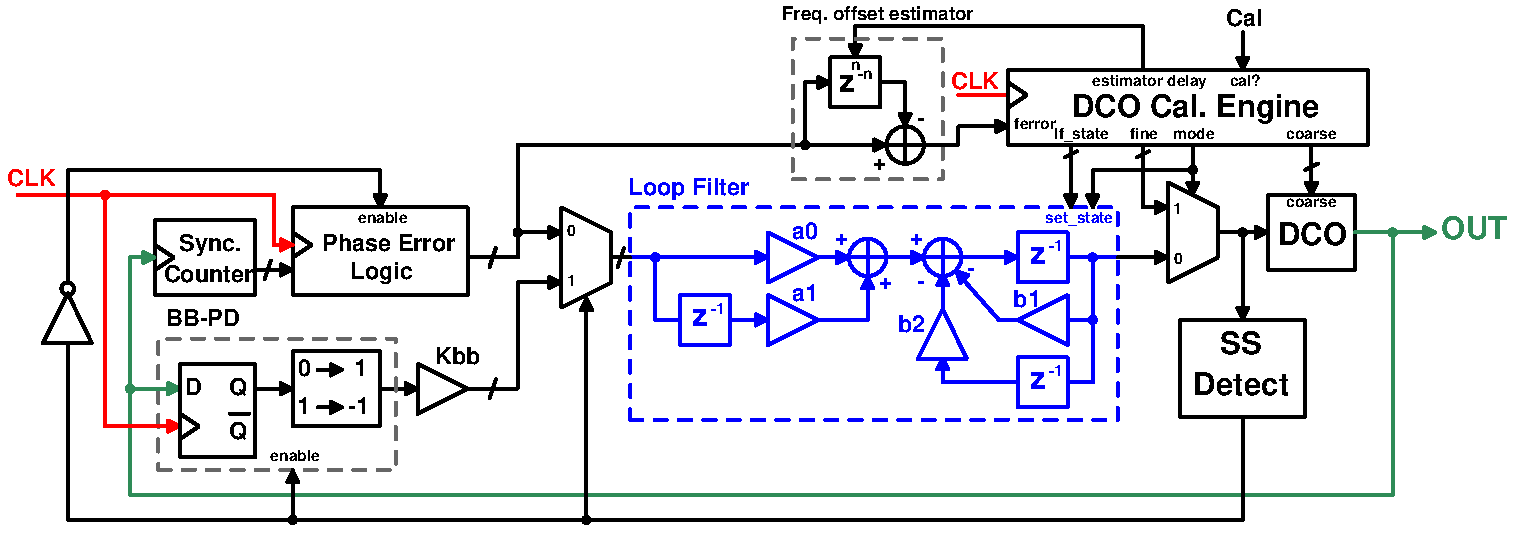
\includegraphics[width=0.8\textwidth, angle=0]{pll_master_arch.pdf}

	\end{block}
		\begin{block}{Power Targets {\color{red}(revised)}}
		\scriptsize
		{\color{red}\textbf{(Divider not necessary)}}
		\vspace{-1em}
		\begin{table}[htb!]
			\tiny
			\centering
			\def\arraystretch{1.5}		
			\setlength\arrayrulewidth{0.75pt}
			\setlength{\tabcolsep}{1em} % for the horizontal padding
			\begin{tabular}{|l|l|l|l|l|l|}
				\hline 
				\rule[-1ex]{0pt}{2.5ex} \cellcolor{gray!40}\textbf{DCO} & \cellcolor{gray!40}\textbf{Phase detector} & \cellcolor{gray!40}\textbf{Divider }& \cellcolor{gray!40}\textbf{Digital (LF)}& \cellcolor{gray!40}\textbf{Other} & \cellcolor{gray!40}\textbf{SUM} \\ 
				\hline 
				\rule[-1ex]{0pt}{2.5ex} 50 $\mu$W& 10 $\mu$W & \textbf{N/A} {\color{red}\st{10 $\mu$W}} & 10 $\mu$W  & $\leq$ \textbf{5} {\color{red}\st{10}} $ \mu$W & $\leq$ \textbf{75} {\color{red}\st{100}} $\mu$W\\ 
				\hline 
			\end{tabular} 
			% \caption{Assigned specifications for branch line hybrid design.}
			% \label{asgn_specs}
		\end{table}   
	\end{block}

\end{frame}

% #############################################################################
% Specification
% #############################################################################

\begin{frame}
	\frametitle{Specification\color{black}}
	\begin{block}{System Performance Targets}
		\tiny
		\begin{table}[h!]
			\centering
			\def\arraystretch{1.5}		
			\setlength\arrayrulewidth{0.75pt}
			\setlength{\tabcolsep}{1em} % for the horizontal padding
			\begin{tabular}{|l|r|l|l|}
				\hline 
				\rule[-1ex]{0pt}{2.5ex} \cellcolor{gray!40}\textbf{Parameter} & \cellcolor{gray!40}\textbf{Value} & \cellcolor{gray!40}\textbf{Unit }& \cellcolor{gray!40}\textbf{Notes}\\ 
				\hline 
				\rule[-1ex]{0pt}{2.5ex} \textbf{Frequency}  & 2.4-2.4835 & GHz & 2.4G ISM Band\\ 
				\hline 
				\rule[-1ex]{0pt}{2.5ex} \textbf{Ref. frequency} & 16 & MHz & Yields 6 channels \\ 
				\hline 
				\rule[-1ex]{0pt}{2.5ex} \textbf{Power} & $\leq$ \textbf{75} {\color{red}\st{100}} $\mu$W  &$\mu$W & Minimize!\\ 
				\hline 
				\rule[-1ex]{0pt}{2.5ex} \textbf{FSK BER} & $\leq$ 1e-2  & & GFSK\textbf{*} with $f_{dev}$=$\pm$250 KHz\\ 
				\hline 
				\rule[-1ex]{0pt}{2.5ex} \textbf{CNR} & $>$ 20 & dBc&Yields  \textbf{-235} {\color{red}\st{-233}} dB FOM$_{jitter}$ ideally \\ 
				\hline 
				\rule[-1ex]{0pt}{2.5ex} \textbf{Initial Lock Time} & $\leq$ 10 & $\mu$s & Upon cold start \\ 
				\hline 
				\rule[-1ex]{0pt}{2.5ex} \textbf{Re-lock Time} & $\leq$ 5 & $\mu$s & Coming out of standby, $f_{error} <$ \textbf{1 MHz} \\ 
				\hline 
				\rule[-1ex]{0pt}{2.5ex} \textbf{Lock $\Delta f$ tolerance} & $100$ & kHz& \\ 
				\hline 
				\rule[-1ex]{0pt}{2.5ex} \textbf{FOM}$_{\textnormal{jitter}}$ & $\leq$ -230 & dB & \textbf{For state of art in size/power} \\ 
				\hline 
				\rule[-1ex]{0pt}{2.5ex} \textbf{Area} & $<$ 0.01  & mm$^2$ & \\ 
				\hline 
			\end{tabular} 
			% \caption{Assigned specifications for branch line hybrid design.}
			% \label{asgn_specs}
		\end{table}   
		\textbf{*} Using BT=0.3, 1 MSymbols/s, 4 demodulated symbols averaged per bit to yield 250 kbps.
	\end{block}    
\end{frame}



\begin{frame}
	\frametitle{Specification\color{black}}
	\begin{block}{Component-level specs}
		\scriptsize
	\begin{table}[h!]
		\centering
		\tiny
		\def\arraystretch{1.5}		
		\setlength\arrayrulewidth{0.75pt}
		\setlength{\tabcolsep}{1em} % for the horizontal padding
		\begin{tabular}{|l|r|l|}
			\hline 
			\rule[-1ex]{0pt}{2.5ex} \cellcolor{gray!40}\textbf{Parameter} & \cellcolor{gray!40}\textbf{Value} & \cellcolor{gray!40}\textbf{Unit }\\ 
			\hline 
			\rule[-1ex]{0pt}{2.5ex} \textbf{Counter range}  & 256 steps & coverage of 150-155 \\ 
			\hline 
			\rule[-1ex]{0pt}{2.5ex} \textbf{Divider ratio} & 150-155  & (For non-counter based)\\ 
			\hline 
			\rule[-1ex]{0pt}{2.5ex} {\color{red}\st{\textbf{TDC resolution}}} &{\color{red}\st{$\geq$ 155}}  & {\color{red}\st{steps/reference cycle}}\\ 
			\hline 
			\rule[-1ex]{0pt}{2.5ex} \textbf{DCO gain $K_{DCO}$} & $10^4$ & Hz/LSB \\ 
			\hline 
			\rule[-1ex]{0pt}{2.5ex} \textbf{DCO tuning range} & 10 & MHz \\ 
			\hline 
			\rule[-1ex]{0pt}{2.5ex} \textbf{DCO DAC resolution} & 10 & bit \\ 
			\hline 
			\rule[-1ex]{0pt}{2.5ex} \textbf{DCO Phase noise} &$<$ -80 & dBc/Hz @ $\Delta f=10^6$ Hz, $f_c$ = 2.448 GHz \\ 
			\hline 
			\rule[-1ex]{0pt}{2.5ex} \textbf{DCO Power} & $\leq$ 50 & $\mu$W \\ 
			\hline 
			\rule[-1ex]{0pt}{2.5ex} \textbf{Digital filter word resolution} & $\leq$ 16 & bits (power grows as $\mathcal{O}(n^2)$) \\ 
			\hline 
			\rule[-1ex]{0pt}{2.5ex} \textbf{BB-PD jitter} & $\leq$ 12 & ps$_{\textnormal{rms}}$ \\ 
			\hline 
		\end{tabular} 
		% \caption{Assigned specifications for branch line hybrid design.}
		% \label{asgn_specs}
		\label{design_specs}
	\end{table}   
	\end{block}    
\end{frame}

% #############################################################################
% Timeline
% #############################################################################

\begin{frame}
	\frametitle{Time plan (pt. 1)}
	\begin{table}[htb!]
		\tiny
		\centering
		\vspace{-1em}
		\def\arraystretch{1.5}		
		\setlength\arrayrulewidth{0.75pt}
		\setlength{\tabcolsep}{1em} % for the horizontal padding
		\begin{tabular}{|c|l|l|l|}
			\hline 
			\rule[-1ex]{0pt}{2.5ex}\cellcolor{gray!40}\textbf{Week \#} & \cellcolor{gray!40}\textbf{Dates} &\cellcolor{gray!40}\textbf{Tasks} & \cellcolor{gray!40}\textbf{Outcomes}\\ 
			\hline 
			% \rule[-1ex]{0pt}{2.5ex} \cellcolor{green!20}\textbf{3}&\cellcolor{green!20}13.1 - 19.1 &\cellcolor{green!20}Review PLL Design &\cellcolor{green!20}Refreshed Knowledge\\ 
			% \hline 
			\rule[-1ex]{0pt}{2.5ex}\cellcolor{red!40}\textbf{4}&\cellcolor{red!40}20.1 - 26.1 &\cellcolor{red!40}Finalize high level modeling &\cellcolor{red!40}Component level specification\\ 
			\hline 
			\rule[-1ex]{0pt}{2.5ex}\textbf{5}\cellcolor{red!40}&\cellcolor{red!40}27.1 - 2.2 &\cellcolor{red!40}Establish test bench in Virtuoso &\cellcolor{red!40}With ideal PLL implementation\\ 
			\hline 
			\rule[-1ex]{0pt}{2.5ex}\cellcolor{green!40}\textbf{6}&\cellcolor{green!40}3.2 - 9.2&\cellcolor{green!40}Schem. design: phase detector &\cellcolor{green!40}TDC - flash and counter based \\ 
			\hline 
			\rule[-1ex]{0pt}{2.5ex}\textbf{7}& 10.2 - 16.2& Schem. design: phase detector & Bang-bang phase detector\\ 
			\hline 
			\rule[-1ex]{0pt}{2.5ex}\textbf{8}&17.2 - 23.2& RTL, synthesis, place\&route & Digital loop filter\\ 
			\hline 
			\rule[-1ex]{0pt}{2.5ex}\textbf{9}&24.2 - 1.3& RTL, synthesis, place\&route & Digital loop filter\\ 
			\hline 
			\rule[-1ex]{0pt}{2.5ex}\textbf{10}&2.3 - 8.3& Schem. design: oscillator & Ring DCO\\ 
			\hline 
			\rule[-1ex]{0pt}{2.5ex}\textbf{11}&9.3 - 15.3& Schem. design: oscillator & LC DCO\\ 
			\hline 
			\rule[-1ex]{0pt}{2.5ex}\textbf{12}&16.3 - 22.3& Schem. design: divider  &TSPC + pulse swallow or sync counter?\\ 
			\hline 
			\rule[-1ex]{0pt}{2.5ex}\textbf{13}&23.3 - 29.3&Schem. design: Calibration& RTL/schem. for calibration\\ 
			\hline 
			\rule[-1ex]{0pt}{2.5ex}\textbf{14}& 30.3 - 5.4 &  Flex week - schem. design & Finalize schematic level design\\ 
			\hline 
			\rule[-1ex]{0pt}{2.5ex}\textbf{15}& 6.4 - 12.4& {\color{red}\textbf{Easter}} & - \\ 
			\hline 
			\rule[-1ex]{0pt}{2.5ex}\textbf{16}& 13.4 - 19.4& Layout & Phase detector\\ 
			\hline 
			\rule[-1ex]{0pt}{2.5ex}\textbf{17}& 20.4 - 26.4& Layout & Oscillator\\ 
			\hline 
		\end{tabular}
		\begin{flushleft}\textbf{Legend:} \colorbox{red!20}{\textbf{Done}} \colorbox{green!20}{\textbf{Current}}  \colorbox{blue!20}{\textbf{Revised}}
		% *I will write the report simultaneously with the work.
		\end{flushleft}
		% \caption{Assigned specifications for branch line hybrid design.}
		% \label{asgn_specs}
	\end{table}   
\end{frame}

\begin{frame}
	\frametitle{Time plan (pt. 2)}
	\begin{table}[htb!]
		\tiny
		\centering
		\vspace{-1em}
		\def\arraystretch{1.5}		
		\setlength\arrayrulewidth{0.75pt}
		\setlength{\tabcolsep}{1em} % for the horizontal padding
		\begin{tabular}{|c|l|l|l|}
			\hline 
			\rule[-1ex]{0pt}{2.5ex}\cellcolor{gray!40}\textbf{Week \#} & \cellcolor{gray!40}\textbf{Dates} &\cellcolor{gray!40}\textbf{Tasks} & \cellcolor{gray!40}\textbf{Outcomes}\\ 
			\hline 
			\rule[-1ex]{0pt}{2.5ex}\textbf{18}& 27.4 - 3.5 & Layout & Divider/calibration\\ 
			\hline 
			\rule[-1ex]{0pt}{2.5ex}\textbf{19}& 4.5 - 10.5 & Layout & Finalization/system integration\\ 
			\hline 
			\rule[-1ex]{0pt}{2.5ex}\textbf{20}& 11.5 - 17.5 & Flex week (layout) OR yield improvement & Depending on progress\\ 
			\hline 
			\rule[-1ex]{0pt}{2.5ex}\textbf{21}& 18.5 - 24.5& {\color{blue}\textbf{Report writing}} & \\ 
			\hline 
			\rule[-1ex]{0pt}{2.5ex}\textbf{22}& 25.5 - 31.5& {\color{blue}\textbf{Report writing}} & \\ 
			\hline 
			\rule[-1ex]{0pt}{2.5ex}\textbf{23}& 1.6 - 7.6& {\color{blue}\textbf{Report writing}} & {\color{red}\textbf{Deadline 8.6}}\\ 
			\hline 
		\end{tabular}
		\begin{flushleft}\textbf{Legend:} \colorbox{red!20}{\textbf{Done}} \colorbox{green!20}{\textbf{Current}}  \colorbox{blue!20}{\textbf{Revised}}
		% *I will write the report simultaneously with the work.
		\end{flushleft}
		% \caption{Assigned specifications for branch line hybrid design.}
		% \label{asgn_specs}
	\end{table}   
\end{frame}


% #############################################################################
% project phases
% #############################################################################

% ############################################################################b#
% References
% #############################################################################


\begin{frame}
	\frametitle{References}
		\scriptsize
		[1]  H. Xu and A. A. Abidi, “Design Methodology for Phase-Locked Loops Using Binary (Bang-Bang) Phase Detectors,” IEEE Transactions on Circuits and Systems I: Regular Papers, vol. 64, no. 7, pp. 1637–1650, Jul. 2017.\par
		\vspace{0.5em}
		[2] F. Gardner, “Charge-Pump Phase-Lock Loops,” IEEE Transactions on Communications, vol. 28, no. 11, pp. 1849–1858, Nov. 1980, doi: 10.1109/tcom.1980.1094619.\par
		\vspace{0.5em}
		% [3] Liu, B., Li, Z., Fu, X., Shirane, A., Kurosu, H., Nakane, Y., Masaki, S., Okada, K., Zhang, Y., Qiu, J., Huang, H., Sun, Z., Xu, D., Zhang, H., Wang, Y. and Pang, J. (2020). A Fully-Synthesizable Fractional-N Injection-Locked PLL for Digital Clocking with Triangle/Sawtooth Spread-Spectrum Modulation Capability in 5 nm CMOS. IEEE Solid-State Circuits Letters, pp.1-1.
	% Navid et al. 2005
\end{frame}


\end{document}
